% --- Instruction Tuning for Reasoning Tasks ---
\section{Instruction Tuning for Reasoning Tasks}
\begin{frame}[allowframebreaks]{}
    \LARGE Instruction Tuning for Reasoning Tasks
\framebreak
    \begin{figure}[h]
        \centering
        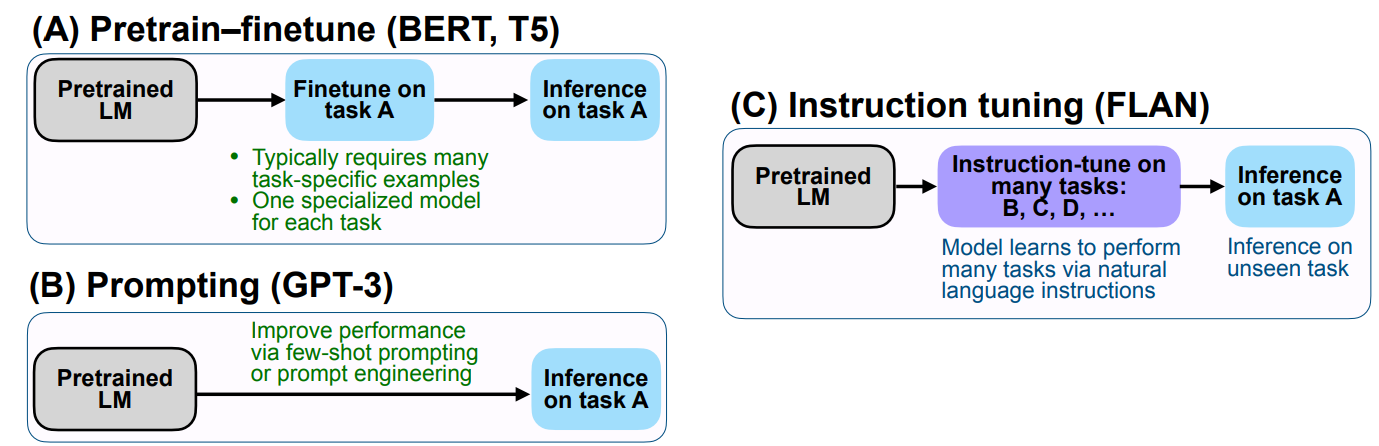
\includegraphics[width=\textwidth,height=0.9\textheight,keepaspectratio]{images/lrm+moe/instruction-tuning.png}
        \caption*{Three ways to use a language model: pretrain--finetune, prompting, and instruction tuning (FLAN). Source: Wei et al. (2022), \href{https://arxiv.org/abs/2109.01652}{arXiv:2109.01652}.}
    \end{figure}
\end{frame}

\begin{frame}[allowframebreaks]{Instruction Tuning}
    \begin{itemize}
        \item \textbf{What is Instruction Tuning?}
        \begin{itemize}
            \item Fine-tuning LLMs on a dataset of instruction-response pairs.
            \item Enhances the model's ability to follow instructions and perform tasks.
        \end{itemize}
        \item \textbf{Why is it important?}
        \begin{itemize}
            \item Improves model performance on diverse tasks.
            \item Enables better generalization to unseen tasks.
        \end{itemize}
    \end{itemize}
    \framebreak
    \begin{block}{Why Instruction Tune LLMs?}
        \begin{itemize}
            \setlength{\itemsep}{0.5em}
            \item Pre-trained LLMs are optimized for next-word prediction, not for following instructions or engaging in conversations.
            \item Without instruction tuning, LLMs may generate text that is linguistically correct but not aligned with user intent.
            \item Instruction tuning uses supervised learning on instruction-response pairs, teaching the model to generate helpful and relevant outputs for user prompts.
            \item Fine-tuning is much more efficient than training a large model from scratch and can be performed with less data and compute.
            \item Instruction tuning bridges the gap between generic language modeling and practical, task-oriented use cases, making LLMs more useful and predictable.
        \end{itemize}
    \end{block}
    \framebreak
    \begin{block}{Summary of Instruction Tuning}
        \begin{itemize}
            \setlength{\itemsep}{1em}
            \item \textbf{Definition:} Fine-tuning LLMs on diverse instruction-response pairs.
            \item \textbf{Key Elements:}
            \begin{itemize}
                \item \textit{Instruction:} Task description in natural language.
                \item \textit{Additional Information:} Optional context or input.
                \item \textit{Desired Output:} Target response for evaluation.
            \end{itemize}
            \item \textbf{Benefits:}
            \begin{itemize}
                \item Improves ability to follow instructions.
                \item Reduces need for prompt engineering and few-shot examples.
                \item Enhances generalization to unseen tasks.
            \end{itemize}
            \item \textbf{Applications:}
            \begin{itemize}
                \item Translation, question answering, reading comprehension, NLI.
                \item Broad improvements across reasoning and practical tasks.
            \end{itemize}
        \end{itemize}
    \end{block}
\framebreak
    \begin{block}{Why Does Instruction Tuning Work?}
        \begin{itemize}
            \item Models learn to \textbf{follow instructions step by step}, rather than just predicting the next word or memorizing answers.
            \item Encourages \textbf{logical reasoning}: Models are guided to explain their answers or show their work, which helps in tasks like math, logic puzzles, and multi-step questions.
            \item \textbf{Generalization:} Instruction-tuned models can handle new types of questions or tasks they have not seen before, simply by following the provided instruction.
            \item \textbf{Variety of Examples:}
            \begin{itemize}
                \item \textit{Math:} ``Solve: What is 15 divided by 3?'' $\rightarrow$ ``5''
                \item \textit{Reasoning:} ``Is a whale a mammal or a fish? Explain your answer.'' $\rightarrow$ ``A whale is a mammal because it gives birth to live young and breathes air.''
                \item \textit{Summarization:} ``Summarize the following paragraph in one sentence.''
            \end{itemize}
        \end{itemize}
    \end{block}
    \framebreak
    \textbf{Challenges and Limitations of Instruction Tuning}
        \begin{itemize}
            \setlength{\itemsep}{1em}
            \item \textbf{Dataset Quality and Diversity:}
            \begin{itemize}
                \item Large, high-quality datasets are costly to create.
                \item Reliance on few open-source datasets may reduce diversity.
            \end{itemize}
            \item \textbf{Bias Propagation:}
            \begin{itemize}
                \item Proprietary LLMs used for instruction generation can spread their biases to open-source models.
            \end{itemize}
            \item \textbf{Evaluation Concerns:}
            \begin{itemize}
                \item Evaluation often uses proprietary models, which may not reveal all biases or limitations.
            \end{itemize}
            \framebreak
            \item \textbf{Superficial Learning:}
            \begin{itemize}
                \item Smaller models may mimic style without true reasoning.
                \item Gains may reflect pattern matching, not understanding.
            \end{itemize}
            \item \textbf{Overfitting to Training Tasks:}
            \begin{itemize}
                \item Evaluation tasks too similar to training can overstate improvements.
            \end{itemize}
            \item \textbf{Key Insight:}
            \begin{itemize}
                \item Improving base model quality is more impactful than just imitating proprietary systems.
            \end{itemize}
        \end{itemize}
\end{frame}
